\documentclass[../../../Main.tex]{subfiles}
\begin{document}
This subsection describes the implementation and reasoning behind localizing the robot's position in the environment. It is assumed that the initial position is known.\\
\\
Goal:
\begin{itemize}
  \item Localize the robot in the environment.
\end{itemize}

\subsubsection{Reasoning}
There are multiple ways of localizing a robot in an environment, and especially when both the map and the initial pose are assumed to be known. The first idea was to use feature extraction and compare what the robot saw through its lidar scanner to the features in the map. This method was tested and discarded. Instead the choice fell between Kalman filtering and particle filtering. The particle filter has been chosen as it is more flexible than the Kalman filter as it does not need to know the initial pose and it can work with an environment represented by an occupancy grid. To compare the particles and their position with the robot's position, ray casting, to determine what the particles see, will be used.

\subsubsection{Implementation}
The particle filter implementation has been split up into two classes; Localization and laserscanner. The particle filter in itself is placed in the Localization class, while the laserscanner is a utility class. \\
\subsubsection*{Laserscanner}
The laserscanner class provides an interface between the lidar and pose data from gazebo and the Localization class.
The laserscanner class provides the functions to perform ray casting on the generated particles.\\
It also provides the three functions that needs to be updated in order for the particle filter to generate a new prediction on the robot's position.
They are updateLidar(), that gets the robot's lidar data (angle and range for all 200 rays that is generated for the robot) and store them in two vectors, updatePos(), that updates the robot's position according to gazebo and lastly updateSpeed(), which gets the robot's angle velocity and speed from gazebo.
This has been done because all three sources of information has to be updated between running the particle filter, or else the particle filter might make its prediction based on old data but compare the estimated particles position with a new Lidar scanning and hence give a false negative.
To ensure the particle filter does not make a new prediction unless new data has been received by laserscanner, each function sets a flag high, and the predict() function in the Localizition class will check if the flag is high or not.\\

The laserscanner class has three other function; rayCasting() performs the ray casting based on an (x,y) coordianteset and the angle\footnote{the ray casting is based on the lidar max range and the angle incrementation of the lidar scanner.} $\beta$ while drawLines() adds the pixels coordinates of each genrated ray to a vector. 200 rays are generated by rayCasting() per particle. The last function, calDistance(), calculates the distance of each ray based on the pixel values given vector from drawLines().
The vector either contains no black pixels and the length will be based on the starting coordinate and the end coordinate or if a black pixel is in the vector, the endpoint will be the black pixel instead of the last element in the vector.
The drawLines() and calDistance() functions are based on Bresenham's line algorithm.\\

It is important to mention, that the lidar data provided by gazebo is given in meters. So a conversion from meters to pixels has to be performed in order for the conversion between the robot's rays and the particles rays to be calculated correctly. It is also worth noting that the robot sees its initial position as (0,0) although it starts in the middle of the map. This will be important later on.

\subsubsection*{Particle filter}
The particle filter is made up of 5 functions with 3 of them being the main functions. A particle filter consists of a prediction function, that makes a prediction based on the former (x,y) coordinate and angle and the speed and angle velocity with which the robot moves, a update function and a resampling function. \\

The prediction function generates 200 particles\footnote{the higher the particle count, the more precise estimate of the location}, and each contains an estimate of where it thinks the robot is.
To ensure that as many possible positions of the robot is covered, the estimates gets a random Gaussian noise added on the speed and angle velocity, see figure \ref{eq:1}.
\begin{figure}[H]
  \begin{equation}
      x_{k+1} = x_k + (v_k + \delta v_k ) \cdot \Delta T \cdot cos(\phi _ k)
  \end{equation}
  \begin{equation}
      y_{k+1} = y_k + (v_k + \delta v_k ) \cdot \Delta T \cdot sin(\phi _ k)
  \end{equation}
  \begin{equation}
      \phi _{k+1} = \phi_k + (\omega _k + \delta \omega _k ) \cdot \Delta T
  \end{equation}
  \caption{ $x_{k+1}$, $y_{k+1}$ and $\phi_{k+1}$ are the predicted next position and direction of the robot. $x_k, y_k, \phi_k$ is the current position in x, y and angle. $v_k and \omega _k$ is the current velocity and angle velocity of the robot. The $\delta \omega _k$ and $\delta v_k$ is the added Gaussian noise.}
   \label{eq:1}
\end{figure}

The first prediction does, however, not occur in prediction(). It is generated in the init function, as the particles needs to be generated along with their weight, last known coordinates and so on, as the prediction function relies on this information to estimate the new position. As the initial position is known, the first particles position will be generated uniformly around this area, see listening \ref{lst:prediction}. This means that a conversion between the (0,0) coordinate provided by gazebo needs to be converted to the middle of the map, else the initial prediction will be way off - as it happened in the first iteration of the particle filter, see figure \ref{fig:particle_filter_initial}.  \\

\begin{lstlisting}[language=C++, caption= Codesippet of the initial prediction of the particles, label={lst:prediction}]
uniform_real_distribution<double> vel_variance(-2.5, 2.5);
    uniform_real_distribution<double> angle_variance(-2.89, 2.89);
    first_flag = true;

    particle p;
    for(int i = 0; i < N; i++)
    {
        r_x = (ls.robot_x + 42)/0.07;
        r_y = ((-1)* ls.robot_x + 20)/0.07;
        //gives all starting particles a random starting point in a 5x5 cube
        double start_x = r_x + vel_variance(gen);
        double start_y = r_y + vel_variance(gen);
        double start_beta = ls.robot_angle + angle_variance(gen);
        current_time = time(&timer);
        p.last_time = current_time;
        p.x = start_x;
        p.y = start_y;
        p.beta = start_beta;
        p.weight = 1/200.0;
        p.likelihood = 0.0;
        // checks if any of the particles are out of the map, if so, it tries again
        if(checkCoordinates(start_x, start_y))
        {
            //update the predicted values and last time.
            samples.push_back(p);
        }
        else
            i--;
\end{lstlisting}

\begin{figure}[H]
  \centering
  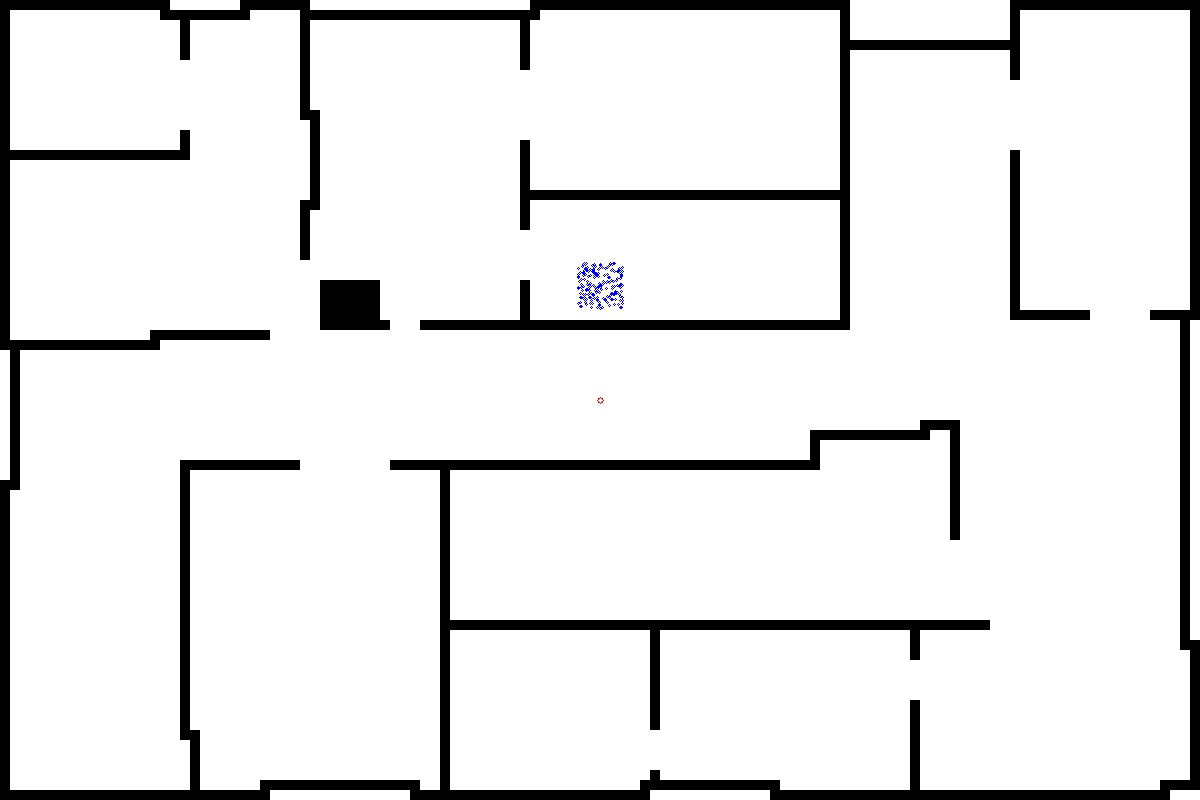
\includegraphics[width=10cm]{\main/afsnit/rob/particle_filter/pictures/newMap.png}
  \caption{The figure shows the initially generated particles, blue circles, and the initial pose of the robot before the conversion mistake was fixed. }
  \label{fig:particle_filter_initial}
\end{figure}
After the prediction function has updated the estimates, it calls the updatePos()\footnote{Not to be confused with updatePose() from laserscanner}.\\

The updatePos() starts by updating a vector variable with the robot's rays lengths\footnote{obtained from gazebo} as well as their relative angle seen as robot.
Next it calls the rayCasting() from Laserscanner to generate the particle rays and get the length for all 200 particles.
Then it calculates the likelihood of every particle being on or very close to the robot's actual location using maximum likelihood. The likelihood is based on the order and length of the particles rays, $\widehat{d_j}$ and the robot's rays $d_j$.
The smaller difference between expected length the particles generate and the actual length the robot see, the more likely it is that the particle is in the right spot.
The likelihood is computed using a Gaussian distribution equation as the sensor noise is assumed to be zero mean and variance $\sigma^{2}$:
\begin{figure}[H]
  \begin{equation}
      \dfrac{1}{\sigma \cdot \sqrt{2 \cdot \pi}} \cdot \exp{- \dfrac{(\widehat{d_j}-d_j)^{2}}{2 \cdot \sigma ^2  }}
  \end{equation}
  \caption{$\widehat{d_j}$ is the expected measurement obtained from the ray casting of each particle and the actual measurement taken from the robot's rays are given by $d_j$ \cite{Guassian}}
\end{figure}
The new weight of all particles are computed based on their likelihood.
The particles weights are normalized afterwards, see listening \ref{lst:label}. updatePos() calls the updateMap() function before the last main function, resamping(). UpdateMap() is purely a help function to visualizes the particles and the robots actual position, see figure \ref{fig:particle_filter_1}.

\begin{lstlisting}[language=C++, caption= Code of likelihood calculation and normliazing of aprticles weight, label={lst:label}]
//calculate the likelihood for a particle is around the robot for all particles.

 double norm_const = 0.0;
 vector<double> temp_weight;
 const double extra = 1/(sigma*sqrt(2*pi));
 double sum = 0;
 for(int i = 0; i < N; i++) // samples size
 {
     double likelihood = 1.0;
     for(int j = 0; j < N; j++) //nranges size - FIX
     {
         likelihood = likelihood * extra *exp(-(pow(samples[i].ray[j].distance-robot_rays[i].distance,2))/(2*pow(sigma,2)));
     }
     //save the likelihood for the particle
     samples[i].likelihood = likelihood;
     //cal new weight based on the likelihood of the particles rays.
     temp_weight.push_back(samples[i].weight * samples[i].likelihood);


     // get the sum of all weights for normalizing.
     norm_const = norm_const + temp_weight[i];
 }
 //normalize new weight of particles
 for(int i = 0; i < N; i++)
 {
     samples[i].weight = temp_weight[i]/norm_const;
     sum= sum + samples[i].weight;
   //  cout << samples[i].weight << endl;

 }
\end{lstlisting}
The function resampling is performed to avoid a small number of highly weighted particles to dominate the estimate of the robot location. It resamples all particles that are not over a certain threshold and make the new particles based on the ones that are over the threshold. All 200 particles will be resampled and get assigned an equal weight in accordance with the pseudo code from our textbook \cite{robbook}.

\begin{figure}[H]
  \centering
  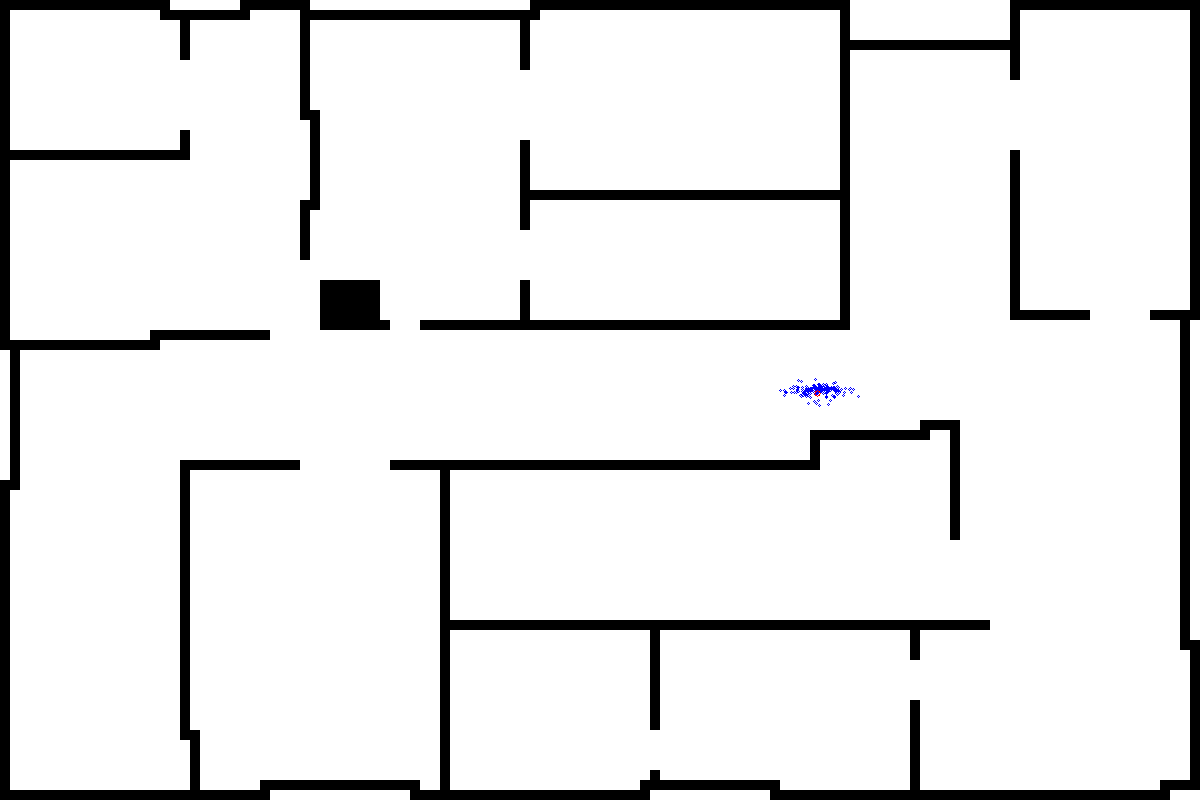
\includegraphics[width=10cm]{\main/afsnit/rob/particle_filter/pictures/particles_moved_1.png}
  \caption{The figure shows the 200 particles, blue circles, following very closely around the actual position of the robot, red circle.}
  \label{fig:particle_filter_1}
\end{figure}

As can be observed on figure \ref{fig:particle_filter_1}, the particles are not spot on the actual position. They are however, fairly close to the actual position. The cluster of particles does not in themselves give an "actual" position of the robot, as it is merely a cluster of estimated positions.
Instead a method to obtaining the most likely position would be taking the average of the particles (x,y) and pick that as the best possible estimate of the location.
The particles generated in the initial prediction appears to be as close to the robot as one might expect.
It does before much more closely clustered the closer to the hallway the robot gets.
It is suspected that this phenomenon occurs because of the uniform distribution used in the initial prediction, see listening \ref{lst:prediction}.
If the position had been unknown from the start, the uniform distribution would have been a good choice, however not with the current bounds used, but as the position IS known, Gaussian would potentially been a better pick.  \\

\begin{figure}[H]
  \centering
  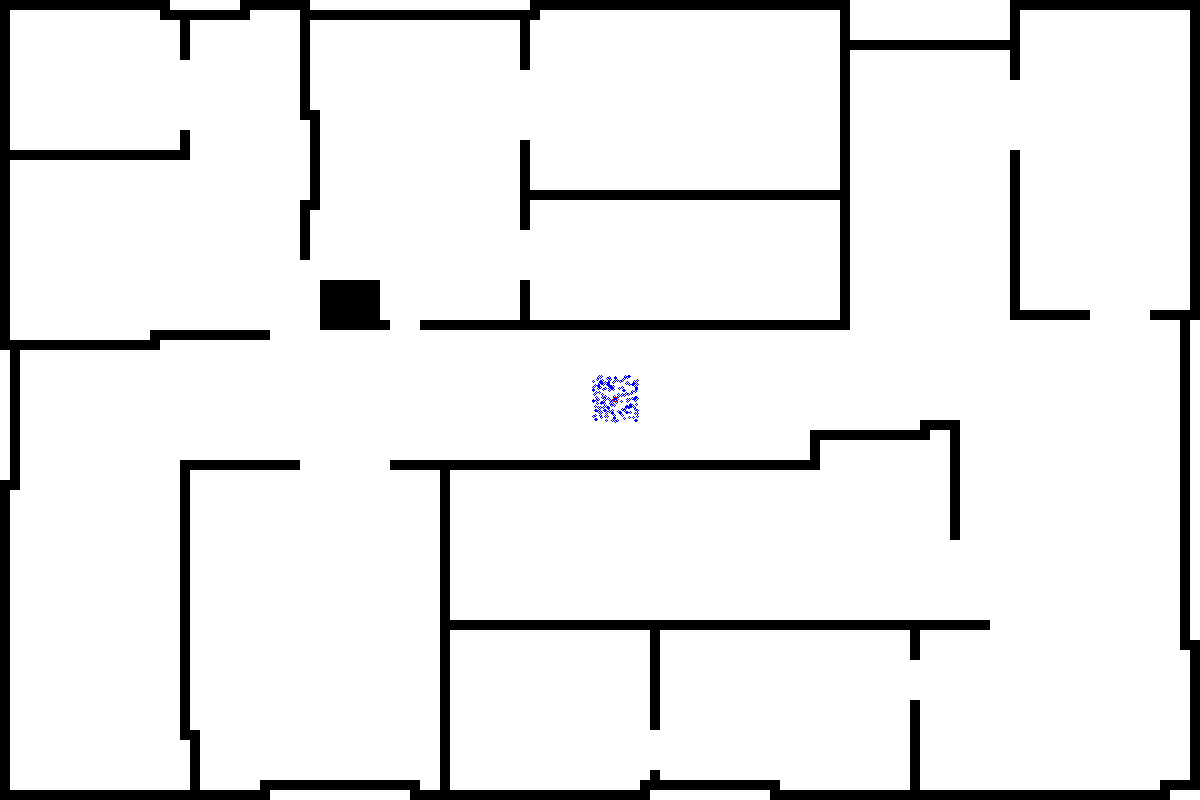
\includegraphics[width=10cm]{\main/afsnit/rob/particle_filter/pictures/int_done_right.png}
  \caption{The figure shows the initial position of the 200 particles, blue dots, and the robot, red dot - using an uniform distribution to generate the particles.}
  \label{fig:particle_filter_1}
\end{figure}

One thing that became apparent was, that if the particles first believes in the wrong particle, it can take quite a long time before it comes back.
There is an issue with the particle filter, if it is used in the map when there is marbles present. This is because only the robot can see the marbles and the lidar scanning are affected as if there is a wall while the particles rays are generated from the provided map, which does not include the marbles. This means, that in a worst case scenario, where the robot is left standing looking at a marble close up, the particles might start migrating and completely miscalculate the location, see figure \ref{fig:u_fucked}. If the robot moves the particles will eventually find their way back.

\begin{figure}[H]
  \centering
  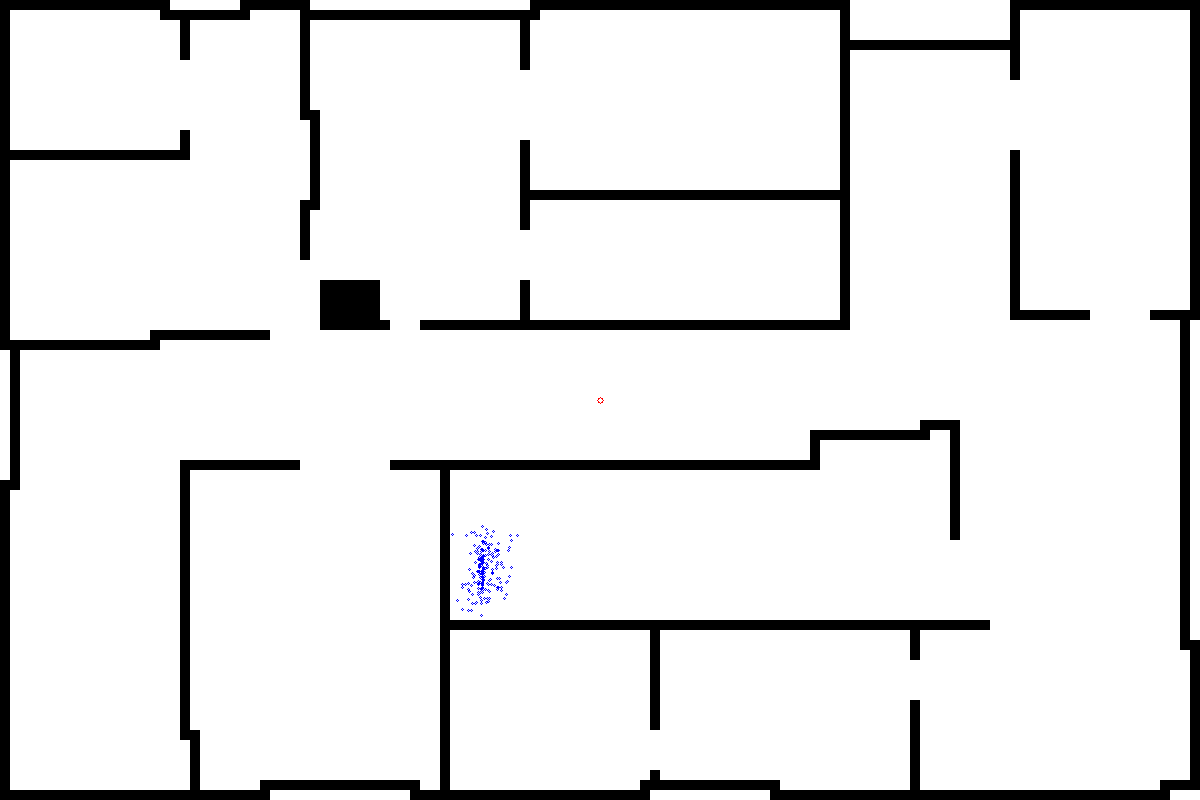
\includegraphics[width=10cm]{\main/afsnit/rob/particle_filter/pictures/try2.png}
  \caption{The figure shows the initial position of the 200 particles, blue dots, and the robot, red dot, not reacting well to a difference in the what the robot sees and what the particles think it should see }
  \label{fig:u_fucked}
\end{figure}
\subsubsection{Conclusion}
The particle filter works quite well, all though it would not yet be suited to actually be used in the map with marbles in it. It could maybe be better to switch out the uniform distribution for a Gaussian in the init() function, however it is not the biggest of issues. More turning using the sigma variable in the most likelihood calculation might solve how spread out the particles are in figure \ref{fig:particle_filter_1}.
\end{document}
